%%%%%%%%%%%%%%%%%%%%%%%%%%%%%%%%%%%%%%%%%%
%Copyright (C) 2018-2019 YuZJ Lab.
%使用CC-BY-NC-SA授权。一份完整版本的许可证已位于附录。这个版本原始作者YuZJ,
%邮箱\theafamily@126.com(最后连接于2019年06月20日17:32:17)。
%%%%%%%%%%%%%%%%%%%%%%%%%%%%%%%%%%%%%%%%%%
\section{高级反病毒技巧}
当一般的反病毒软件无法将病毒清除时,你就应该考虑使用病毒移除工具或使用GNU/Linux反病毒\footnote{当然你也可以重装系统。但这么做无法清除系统盘以外的病毒。}。
\subsection{病毒移除工具:以KVRT为例}
我们仍然使用卡巴斯基病毒移除工具(Kaspersky Virus Removal Tool,KVRT)演示它们的使用。下载:\url{https://www.kaspersky.com.cn/downloads/thank-you/free-virus-removal-tool}(最后连接于2019年06月20日18:44:31,网速较慢)。
\begin{center}
	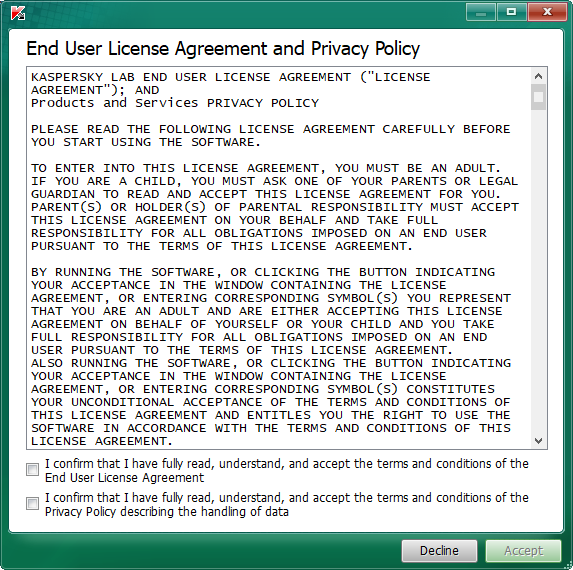
\includegraphics[scale=0.5]{pic/kvrt_eula.PNG}        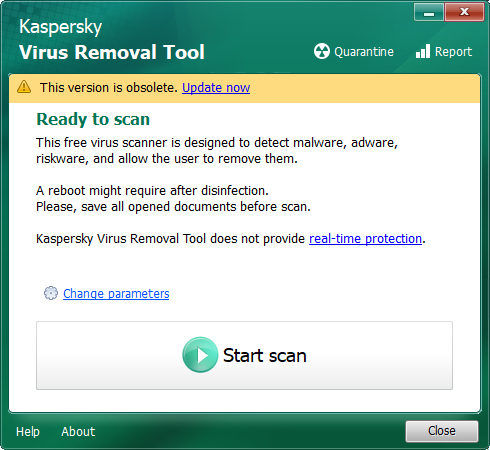
\includegraphics[scale=0.6]{pic/kvrt_ready.PNG}\\
	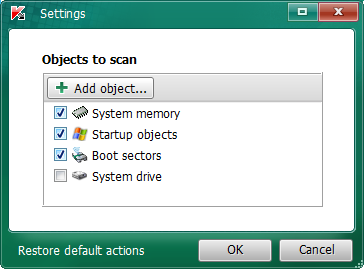
\includegraphics[scale=0.6]{pic/kvrt_conf.PNG}
	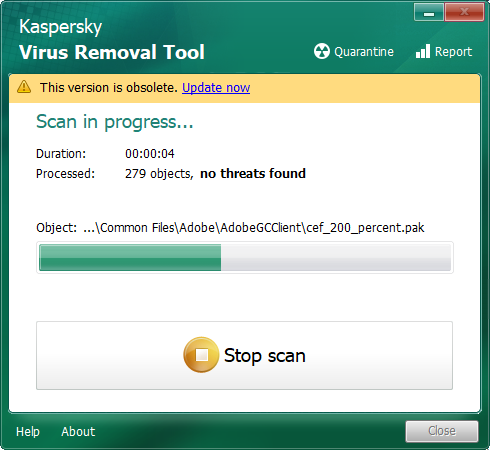
\includegraphics[scale=0.4]{pic/kvrt_ing.PNG}    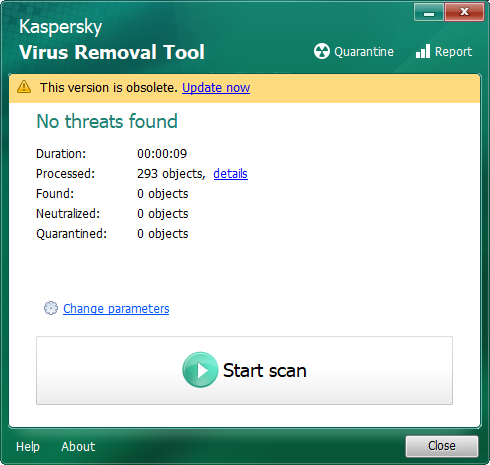
\includegraphics[scale=0.4]{pic/kvrt_compl.PNG}
\end{center} \par
上图分别是KVRT显示最终用户许可声明及隐私保护条例,准备查杀,配置扫描范围,正在查杀,查杀完成的界面。\par
首先你应该同意最终用户许可声明及隐私保护条例(注意,你首先应该看过它)。选中两个复选框再单击“Accept”即可。之后它会“初始化”(initialization)一段时间,并显示“准备好”界面\footnote{注意到上面黄色的一块区域了吗?它的出现说明这个版本已经过时了,你可以选择重新下载最新版。}。\par
现在选择查杀范围。单击“change parameters”,你将发现图3所示对话框。其中“System memory”指“系统内存”,“Startup objects”指启动项,“Boot sectors”指启动扇区,“System drive”指系统盘(一般是“C:\textbackslash”)。你还可以单击“Add object”添加其它文件或磁盘。\par
单击“Start scan”开始扫描\footnote{需要消耗一(大)段时间并占用大量系统资源}。
\subsection{使用以GNU/Linux为操作系统的计算机急救工具}
GNU/Linux可用于Windows反病毒原因是:Windows二进制文件与GNU/Linux二进制文件的结构是不同的(具体请参考其他专业书籍),因此Windows的EXE病毒大多数情况下无法在GNU/Linux上运行(使用Wine \footnote{一种类似于虚拟机的技术,它可允许Windows应用程序在GNU/Linux,BSD等操作系统上运行。} 或其他类似技术除外),也就是说,Windows下的病毒一般无法感染GNU/Linux操作系统。\par
大多数反病毒软件厂商都提供了“急救盘”,用于给无法启动或严重感染的计算机反病毒。大多数急救盘基于GNU/Linux \footnote{如Dr.Web和AVIRA基于Ubuntu 14(Dr.Web凭借Wine运行),Kaspersky基于Gentoo Linux x86\_64,ESET基于其它GNU/Linux操作系统。},也有少部分(如Avast!)基于Windows。\par
现将以Kaspersky Rescure Disk以演示GNU/Linux反病毒。至于如何安装GNU/Linux并反病毒请参见\pageref{sec:avgl}页\ref{sec:avgl}\par
现在你将计算机开启,将光盘插入光驱后重启。你将被引导到光盘启动。你将发现:
\begin{center}
	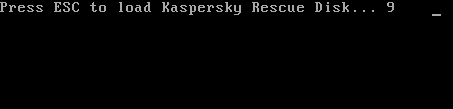
\includegraphics[scale=0.7]{pic/krd1}
\end{center} \par
此时,快速按下ESC键(它应位于你键盘左上角),进入左图所示界面,选择“English”--英语,敲击回车,进入右图界面。此时你应该选择“Kaspersky Rescure Disk, Graphic Mode”(图形界面)\footnote{下面“Limited graphic mode”为限制的图形界面,“Hardware info”为探测硬件信息,“Boot from hard disk”为从硬盘启动(意思就是说,启动硬盘里已经安装的操作系统),“Reboot”与“Shutdown”指重启与关机。当然高手请随意。}
\begin{center}
	
\includegraphics[scale=0.25]{pic/krd2}	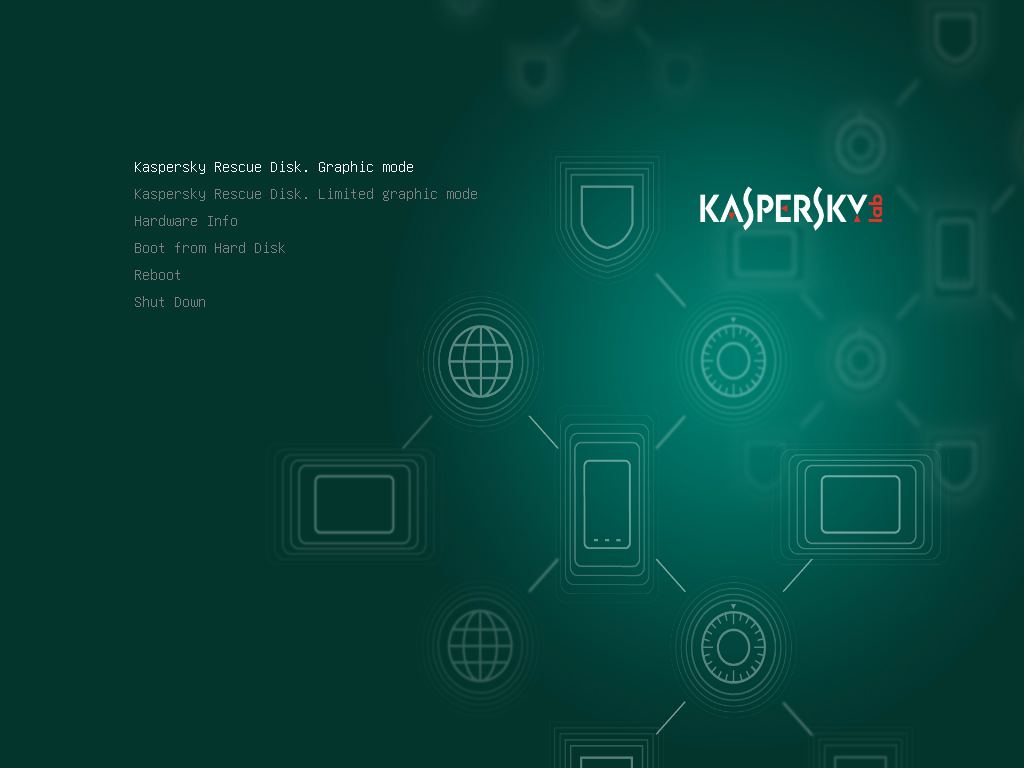
\includegraphics[scale=0.25]{pic/krd3}
\end{center} \par
这就启动好了。KRD提示你整个系统正在内存上运行,所有新病毒库、日志、隔离等在关机后都将丢失。之后你会看见右图界面,是不是很熟悉呢?
\begin{center}
	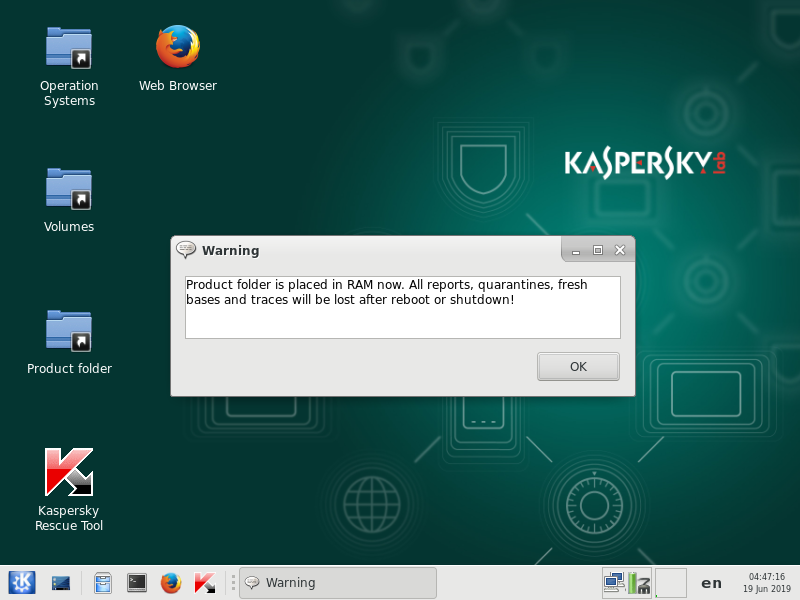
\includegraphics[scale=0.35]{pic/krd4}	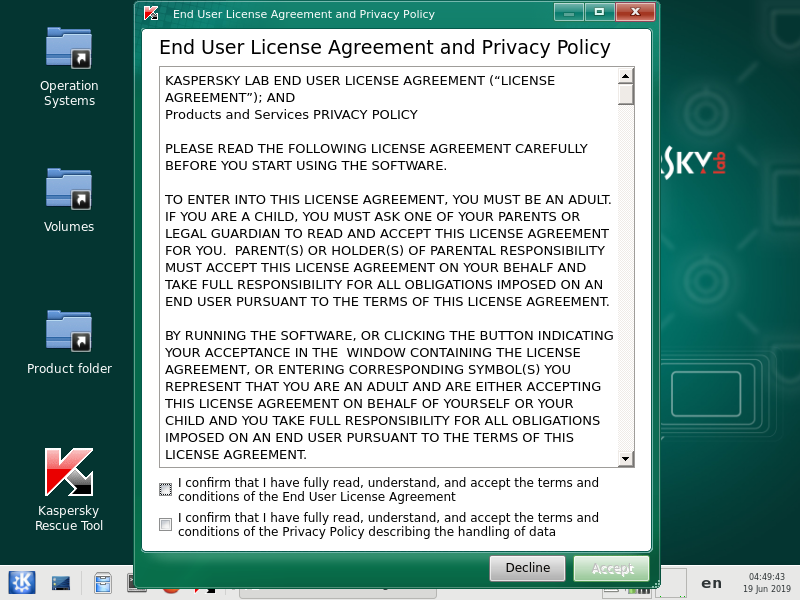
\includegraphics[scale=0.35]{pic/krd5}
\end{center} \par
除了反病毒,KRD还提供了网络浏览器Firefox、终端、任务管理器Htop与Task Manager(参见\pageref{sec:pm}页\ref{sec:pm})、图像查看器Ristretto Imagine Viewer、文件管理器Midnight Commander与Thunar File Manager、文本编辑器Mousepad等。默认以root用户登录。其余设置较为复杂,请参照“高级”章。
